\begin{figure}[bth!]
	\begin{center}
		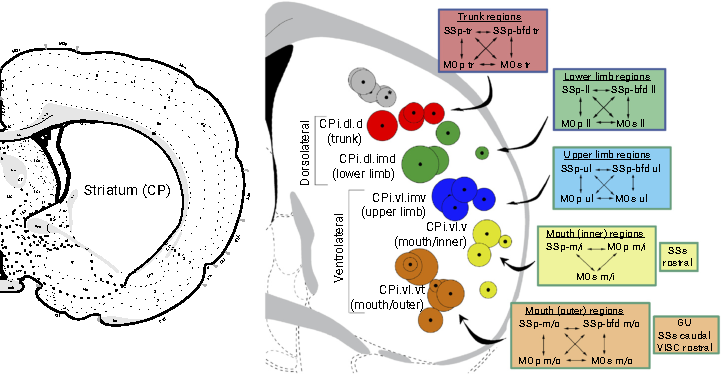
\includegraphics[width=1\linewidth]{ch-intro/figures/StriatumInputMap}
		\caption[Map of Cortical Inputs to DLS]
		{\textbf{Somatotopic map of cortical inputs to the \gls{dls}.}
		\textit{Left}:~striatum (CP) in the rat brain atlas.
		\textit{Right}:~inputs from somatosensory cortices form a topographic map in the \gls{dls}.
		CPi:~the intermediate portion of the striatum along the rostrocaudal axis (other abbreviations are defined in the original reference and are not important here).
		Figure adopted from~\cite{Hintiryan2016NN}.
		}
		\label{fig:intro:InputMap}
	\end{center}
\end{figure}